\documentclass[a4paper,12pt]{article} % добавить leqno в [] для нумерации слева
\usepackage[a4paper,top=1.3cm,bottom=2cm,left=1.5cm,right=1.5cm,marginparwidth=0.75cm]{geometry}
%%% Работа с русским языком
\usepackage{cmap}					% поиск в PDF
\usepackage{mathtext} 				% русские буквы в фомулах
\usepackage[T2A]{fontenc}			% кодировка
\usepackage[utf8]{inputenc}			% кодировка исходного текста
\usepackage[english,russian]{babel}	% локализация и переносы

\usepackage{graphicx}
\usepackage{mathtools}
\usepackage{wrapfig}
\usepackage{tabularx}
\usepackage{amssymb}
\usepackage{hyperref}
\usepackage[rgb]{xcolor}
\hypersetup{colorlinks=true,urlcolor=blue}
%% Шрифты
\usepackage{euscript}	 % Шрифт Евклид
\usepackage{amsmath}
\usepackage{mathtools}
%%% Заголовок
\author{Lokhmatov Arseniy}
\title{Лабораторная работа по общей физике}

\date{\today}
\begin{document}
\begin{titlepage}
    \newpage
    \begin{center}
    {\large МОСКОВСКИЙ ФИЗИКО-ТЕХНИЧЕСКИЙ ИНСТИТУТ (НАЦИОНАЛЬНЫЙ ИССЛЕДОВАТЕЛЬСКИЙ УНИВЕРСИТЕТ)}
    \vspace{1cm}

    {\largeФизтех-школа аэрокосмических технологий}
    \vspace{6em}
    \end{center}
    
    \vspace{1.2em}

    \begin{center}
    %\textsc{\textbf{}}
    \Large Лабораторная работа №3.4.2 \\
    Закон Кюри-Вейсса 
    \linebreak
    \end{center}
    
    \vspace{11em}
    
    \begin{flushright}
                       {\large Работу выполнил\\
                       Лохматов Арсений Игоревич\\
                       Козярский Алексей Сергеевич\\
                       Дудин Иван Юрьевич\\
                       Б03-303 }
    \end{flushright}

    \vspace{\fill}

    \begin{center}
        
\includegraphics[width=0.2\linewidth]{dasr.png}
    \end{center}

    \begin{center}
    Долгопрудный, 2024
    \end{center}

    \end{titlepage}

\section{Теоретическая часть}

\paragraph{Цель работы:} проверить экспериментально закон Кюри-Вейсса.

\paragraph{Оборудование:} катушка самоиндукции с образцом из гадолиния, термостат, частотометр, цифровой вольтметр, $LC$-автогенератор, термопара медь-константан.

\subsection{Экспериментальная установка}

Схема установки Для проверки закона Кюри-Вейсса изображена на рисунке \ref{img1}. Исследуемый ферромагнитный образец (гадолий) расположен внутри пустотелой катушки самоиндукции, которая служит индуктивностью колебательного контура, входящего в состав $LC$-автогенератора. Автогенератор собран на полевом транзисторе и смонтирован в виде отдельного блока.

\begin{figure}[h]
\begin{center}
		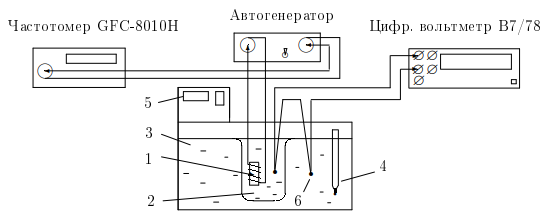
\includegraphics[width=18cm]{card1.png}
\end{center}
	\caption{Схема установки}
	\label{img1}
\end{figure}

Гадолиний -- хороший проводник электрического тока, а рабочая частота генератора достаточно велика, порядка $\sim 50 \text{ кГц}$, поэтому для уменьшения вихревых токов образец изготовлен из мелких кусочков. Катушка $1$ с образцом помещена в стеклянный сосуд $2$, залитый трансформаторным маслом. Масло предохраняет образец от окисления и способствует ухудшения электрического контакта между отдельными кусочками образца. Также оно улучшает тепловой контакт между образцом и рабочей жидкостью $3$ в термостате. Ртутный термометр $4$ используется для приближённой оценки температуры.

При изменении температуры меняется магнитная восприимчивость образца $\chi$, а следовательно, самоиндукция катушки и период колебаний $\tau$ автогенератора. Для измерения периода используется частотометр.

\textbf{Закон Кюри-Вейсса} справедлив, если выполнено соотношение 

\[ \frac{1}{\chi} \sim (T - \theta_{p}) \sim \frac{1}{(\tau^2-\tau^2_{o})}, \]

где $\tau_{o}$ -- период колебаний в отсутствии образца.

Температура исследуемого образца всегда несколько отличается от температура дистиллированной воды в сосуде. После того как вода достигла заданной температуры , идёт медленный процесс стабилизации температур образца и воды. Разность их температур контролируется с помощью медно-константановой термопары $6$ и цифрового вольтметра. Один из спаев термопары находится в тепловом контакте с образцом, а другой погружён в воду. Концы термопары подлючены к цифровому вольтметру. Рекомендуется измерять период колебаний автогенератора в тот момент, когда указанная разность температур становится $\leq0.5 \text{ } C^{\circ}$. Чувствительность термопары $k = 24 \text{ Град}/\text{мВ}.$

\section{Практическая часть}

В работе предлагается измерить зависимость периода колебаний автогенератора от температуры сердечника катушки и по результатам измерений определить парамагнитную точку Кюри гадолиния.

\subsection{Подготовка приборов к работе}

\begin{enumerate}
    \item Убедились, что термостат охлаждён и готов к работе. Включем в сеть автогенератор. Включим частотометр, выберем чувствительность входного канала $1/1$, установим режим измерения периода. Включим вольтметр для измерения напряжения постоянного тока.
    \item Оценим допустимую ЭДС термопары, если длпустимая разница температур образца и рабочей жидкости $\Delta T = 0.5 C^{\circ}$, а постоянная термопары $k = 24 \frac{\text{град}}{\text{мВ}}$. 
    
    В результате получаем, что измерения проводим, когда вольтметр показывает напряжение 
    
    \[U \leq \frac{0.5}{24} = 0.02 \text{ мВ}.\]
    
\end{enumerate}

\subsection{Измерения}

\begin{enumerate}
    \item Исследуем периода колебаний $LC$-генератора от температуры образца, отмечая период колебаний $\tau$ по частотометру, а температуру $T$ - по показанию дисплея термостата.

    Проведём измерения в диапазоне от $14 \text{ } C^{\circ}$ до $40 \text{ } C^{\circ}$ через $2 \text{ } C^{\circ}$. Результаты занесём в таблицу \ref{tab1}.

    \begin{table}[h]
	\centering
	\begin{tabular}{|c|c|c|}
		\hline
		& $ \tau, \text{ } \cdot 10^{-6} \text{ с}$ & $ T, \text{ } C^{\circ}$ \\ \hline
		1 & 7.931 & 14.09 \\ \hline
            2 & 7.87 & 16.10 \\ \hline
            3 & 7.768 & 18.08 \\ \hline
            4 & 7.611 & 20.08 \\ \hline
            5 & 7.438 & 22.05 \\ \hline
            6 & 7.21 & 24.08 \\ \hline
            7 & 7.142 & 26.04 \\ \hline
	\end{tabular}
        \begin{tabular}{|c|c|c|}
		\hline
		& $ \tau, \text{ } \cdot 10^{-6} \text{ с}$ & $ T, \text{ } C^{\circ}$ \\ \hline
		8 & 7.09 & 28.07 \\ \hline
            9 & 7.063 & 30.05 \\ \hline
            10 & 7.044 & 32.05 \\ \hline
            11 & 7.027 & 34.08 \\ \hline
            12 & 7.018 & 36.06 \\ \hline
            13 & 7.01 & 38.03 \\ \hline
            14 & 7.003 & 40.06 \\ \hline
	\end{tabular}
        
	\caption{Результаты измерений}
	\label{tab1}
    \end{table}

    Запишем период колебаний $\tau_{o}$ без образца, указанный на установке.

    \[ \tau_{o} = 6.9092 \text{ } \cdot 10^{-6} \text{ c.} \]

    \item Закончив измерения, отключили все приборы.
    
\end{enumerate}

\subsection{Обработка результатов}

\begin{enumerate}
    \item Поскольку $\Delta T = 0.5 C^{\circ} \ll T$, то в качестве температуры образца будем считать равной температуре термостата.

    \item Построим график $(\tau^2-\tau_{o}^2)=f(T)$, покажем на нём точку Кюри.
\end{enumerate}

\end{document}
